\paragraph{Online Dictionary Examples} We have chosen some well-known, freely accessible online dictionaries that were used in various research
fields.

%%%%%%%%%%%%%%%%%%%%%%%%%%%%%%%%%%%%%%%%%%%%%%%%%%%%%%%%%%WordNet%%%%%%%%%%%%%%%%%%%%%%%%%%%%%%%%%%%%%%%%%%%%%%%%%%%%%%%%%%%%
Started as a research project in 1985 at Princeton University \textbf{WordNet}~\cite{fellbaum1998} is best characterised as a dictionary browser rather than just an online dictionary. It allows users to explore its contents on the basis of semantic, rather than alphabetic similarities. Users look up information along more than one path, semantics being among them. How one wants to explore the possibilities of online dictionaries rather depends on one's ideas and applications one has in mind. 

The building blocks of WordNet are \textit{synsets} which are defined as sets of words having similar semantics~(synonymy). It is important that synonymy does not entail unrestricted interchangeability. By that criterion natural languages would have very few synonyms. Instead, synonymy is typically relative to a context which is encoded as links between and within synsets. 
Several linguistic relations are defined in WordNet, for example \textit{polysemy/monosemy}, \textit{hyponymy/hypernymy} and \textit{meronymy/holonymy}. 
Polysemy/Monosemy describes the fact that a word may have multiple meanings or one meaning. Hyponymy/Hypernymy means that words or phrases are included in the meaning of another word. Meronymy/Holonymy describes part-of or member-of relationships.

The WordNet architecture~\cite{fellbaum1998} as illustrated in~\hyperref[fig:wordnet_architecture]{Figure~\ref*{fig:wordnet_architecture}} can be split into these parts:
\begin{enumerate}
		\item Lexical Source Files
		\item the Grinder
		\item the Lexical Database
		\item Software Tools and Interfaces
\end{enumerate}

\begin{figure}
	 \centering
	 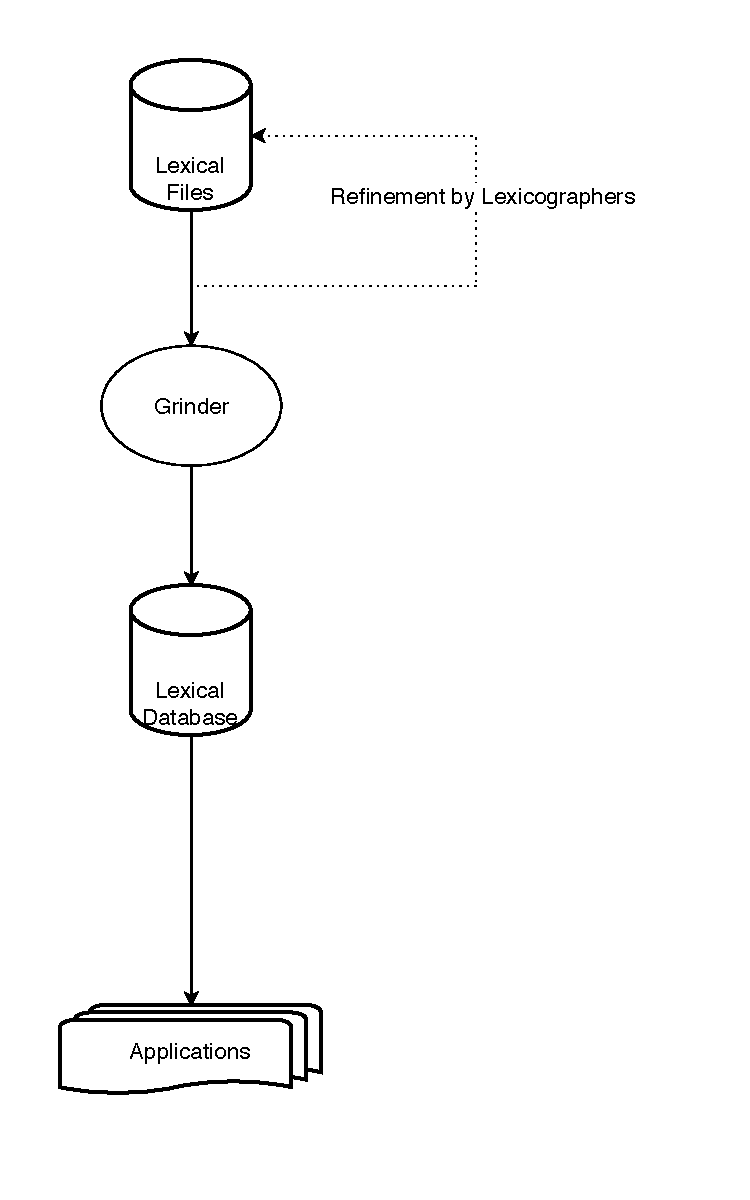
\includegraphics[width=0.5\textwidth]{drawio/WordNet_Architecture}
	 \caption{The architecture of the WordNet System~\cite{fellbaum1998}}\label{fig:wordnet_architecture}
\end{figure}


The \textit{Lexical Database} forms the heart of the WordNet system. It is the result of processing all lexical source files. There are many tools available, written in various programming languages like Perl or awk, to interact with the database. 

WordNet offers some \textit{interfaces} to users for interaction. Depending on the area of application there are textual interfaces~(Command Line Interfaces and APIs) and graphical interfaces~(Desktop Software and Web Applications). Invoking the search form and starting search tasks can also be done via browser interface\footnote{\url{http://wordnetweb.princeton.edu/perl/webwn} accessed 2018/06/14}.

WordNet's key success factor is its potentials in terms of Natural Language Processing~(NLP). It was also used as information source in many other fields~\cite{morato2004}, these are: Image Retrieval, Information Retrieval, Document Classification, Query Expansion, Machine Translation and Conceptual Disambiguation.


%%%%%%%%%%%%%%%%%%%%%%%%%%%%%%%%%%%%%%%%%%%%%%%%%%%%%%%%%%Wiktionary%%%%%%%%%%%%%%%%%%%%%%%%%%%%%%%%%%%%%%%%%%%%%%%%%%%%%%%%%%%%
\textbf{Wiktionary}\footnote{\url{https://www.wiktionary.org/} accessed 2018/06/15} is a freely accessible, collaborative online lexicon~\cite{granger2012}. Whereas traditional dictionaries are the product of a small group of expert lexicographers, collaboratively constructed dictionaries are created by many, not necessarily expert users. This has the advantage that new lexical entries are added more frequently and existing ones are continuously updated. Users are encouraged to participate in content creation and maintenance. New lexical entries are discussed in the community until a consensus is reached. 

An important goal of Wiktionary is openness towards multilingualism. It was first launched in 2002 and indented as an "add-on" to Wikipedia\footnote{\url{https://www.wikipedia.org/} accessed 2018/06/16}. At that time it was only available in English, but now translations exist for nearly every spoken language. However, they differ in scope and community size. Each Wiktionary is accessible by prepending the respective ISO~639~language~code\footnote{\url{https://www.iso.org/iso-639-language-codes.html} accessed 2018/06/16} to the common wiktionary domain.

Content is organised as collections of pages, each containing a title and a body. There are four page categories:
\begin{inparaenum}[1)]
		\item Article Pages,
		\item Redirect Pages,
		\item Talk Pages and
		\item Internal Pages
\end{inparaenum}.
Most pages are \emph{Article Pages}, containing the actual linguistic information. With \emph{Redirect Pages}, users are able to navigate from page to page. At page creation, \emph{Talk Pages} help editors in collecting ideas, expressing criticism, asking questions and discussing page contents. \emph{Internal Pages} are protected and contain motivational information, goals, statistics, indices, appendices and guidelines for contributors. 

Wiktionary is not targeted to specific groups of people nor its content serves a specific purpose, instead, it is open for everyone. 
Linguistic knowledge is organised in separate sections as explained in the next paragraphs: 

It may sound surprising that each page starts with the \emph{language} of the term or phrase because each page belongs to a specific translation of Wiktionary anyway. However, this is necessary because the same term can be encoded in multiple languages. For example, the term \texttt{boat} is used in five languages\footnote{\url{https://en.wiktionary.org/wiki/boat} accessed 2018/06/16}. 

The \textit{etymology} section describes origin and history of a word. It helps linguists in exploring linguistic relations such as synonymy/antonymy, hypernymy/hyponymy and homonymy/polysemy. They are also interested, whether and how the meaning has changed over time. 

\textit{Phonetic references} are appreciated not only by language learners but also by readers who are unfamiliar with particular terms. The term's pronunciation is encoded using audio samples or phonetic notations. 

In contrast to other dictionaries which focus on canonical word forms, Wiktionary also contains entries for inflected word forms. For example, the English verb \texttt{go} and its \textit{morphology} \texttt{went} are encoded as separate entries. Additionally, it may include the declension of an adjective or the conjunction of a verb.

Each term is associated with a \textit{syntactic category} which includes part of speech tags for single words, idioms, proverbs and multi-word expressions. Apart from these, there are also other tags available. For example, nouns are marked as countable/uncountable or singular/plural. 

The most interesting part for dictionary readers is probably the section \textit{semantic knowledge} which describes the meaning of a term. It includes example sentences, quotations, links to other terms, glosses and linguistic labels. The gloss of a word is either a marginal or interlinear notation of the word's meaning. Non-linguists are eventually more familiar with the term \emph{glossary} which denotes to collections of glosses. 

\textit{Cross-lingual knowledge} is especially important for translators and educators who are interested in multilingual realtions. This is expressed as links between pages of differing language. For example, descriptions of the English word \texttt{boat} are contained in a page with links to \texttt{water~craft}, \texttt{full-house} and conformation to \texttt{cyclohexane}.

A valuable feature for non-native speakers is \emph{graphical knowledge}. It is obvious that humans grasp the meaning of a term faster by just looking at a picture or photograph than reading through long textual descriptions. Unfortunately, not all terms can be expressed in pictures or photographs though. 

From a technical perspective Wiktionary is based on MediaWiki\footnote{\url{https://www.mediawiki.org/wiki/MediaWiki} accessed 2018/06/17}, a free and open source software written in PHP\footnote{\url{http://www.php.net/} accessed 2018/06/17}. The software is distributed under the GNU~General~Public~License~(GPL) and maintained by the WikiMedia~Foundation\footnote{\url{https://wikimediafoundation.org/wiki/Home} accessed 2018/06/17}, a non-profit organisation aimed at supporting free, multilingual, educational content. MediaWiki is also used by many other wikis\footnote{\url{https://wikistats.wmflabs.org/} accessed 2018/06/17}.

The majority of wiki features are accessible via public API. Clients can request features or send commands over the \textit{MediaWiki~Action~API}\footnote{\url{https://www.mediawiki.org/wiki/API:Main_page} accessed 2018/06/17}. It has querying, searching, parsing and manipulation capabilities.
